\documentclass[conference]{IEEEtran}

% *** GRAPHICS RELATED PACKAGES ***
%
\ifCLASSINFOpdf
  % \usepackage[pdftex]{graphicx}
  % declare the path(s) where your graphic files are
  % \graphicspath{{../pdf/}{../jpeg/}}
  % and their extensions so you won't have to specify these with
  % every instance of \includegraphics
  % \DeclareGraphicsExtensions{.pdf,.jpeg,.png}
\else
  % or other class option (dvipsone, dvipdf, if not using dvips). graphicx
  % will default to the driver specified in the system graphics.cfg if no
  % driver is specified.
  % \usepackage[dvips]{graphicx}
  % declare the path(s) where your graphic files are
  % \graphicspath{{../eps/}}
  % and their extensions so you won't have to specify these with
  % every instance of \includegraphics
  % \DeclareGraphicsExtensions{.eps}
\fi
% graphicx was written by David Carlisle and Sebastian Rahtz. It is
% required if you want graphics, photos, etc. graphicx.sty is already
% installed on most LaTeX systems. The latest version and documentation
% can be obtained at:
% http://www.ctan.org/pkg/graphicx
% Another good source of documentation is "Using Imported Graphics in
% LaTeX2e" by Keith Reckdahl which can be found at:
% http://www.ctan.org/pkg/epslatex
%
% latex, and pdflatex in dvi mode, support graphics in encapsulated
% postscript (.eps) format. pdflatex in pdf mode supports graphics
% in .pdf, .jpeg, .png and .mps (metapost) formats. Users should ensure
% that all non-photo figures use a vector format (.eps, .pdf, .mps) and
% not a bitmapped formats (.jpeg, .png). The IEEE frowns on bitmapped formats
% which can result in "jaggedy"/blurry rendering of lines and letters as
% well as large increases in file sizes.
%
% You can find documentation about the pdfTeX application at:
% http://www.tug.org/applications/pdftex





% *** MATH PACKAGES ***
%
%\usepackage{amsmath}
% A popular package from the American Mathematical Society that provides
% many useful and powerful commands for dealing with mathematics.
%
% Note that the amsmath package sets \interdisplaylinepenalty to 10000
% thus preventing page breaks from occurring within multiline equations. Use:
%\interdisplaylinepenalty=2500
% after loading amsmath to restore such page breaks as IEEEtran.cls normally
% does. amsmath.sty is already installed on most LaTeX systems. The latest
% version and documentation can be obtained at:
% http://www.ctan.org/pkg/amsmath





% *** SPECIALIZED LIST PACKAGES ***
%
%\usepackage{algorithmic}
% algorithmic.sty was written by Peter Williams and Rogerio Brito.
% This package provides an algorithmic environment fo describing algorithms.
% You can use the algorithmic environment in-text or within a figure
% environment to provide for a floating algorithm. Do NOT use the algorithm
% floating environment provided by algorithm.sty (by the same authors) or
% algorithm2e.sty (by Christophe Fiorio) as the IEEE does not use dedicated
% algorithm float types and packages that provide these will not provide
% correct IEEE style captions. The latest version and documentation of
% algorithmic.sty can be obtained at:
% http://www.ctan.org/pkg/algorithms
% Also of interest may be the (relatively newer and more customizable)
% algorithmicx.sty package by Szasz Janos:
% http://www.ctan.org/pkg/algorithmicx




% *** ALIGNMENT PACKAGES ***
%
%\usepackage{array}
% Frank Mittelbach's and David Carlisle's array.sty patches and improves
% the standard LaTeX2e array and tabular environments to provide better
% appearance and additional user controls. As the default LaTeX2e table
% generation code is lacking to the point of almost being broken with
% respect to the quality of the end results, all users are strongly
% advised to use an enhanced (at the very least that provided by array.sty)
% set of table tools. array.sty is already installed on most systems. The
% latest version and documentation can be obtained at:
% http://www.ctan.org/pkg/array


% IEEEtran contains the IEEEeqnarray family of commands that can be used to
% generate multiline equations as well as matrices, tables, etc., of high
% quality.




% *** SUBFIGURE PACKAGES ***
%\ifCLASSOPTIONcompsoc
%  \usepackage[caption=false,font=normalsize,labelfont=sf,textfont=sf]{subfig}
%\else
%  \usepackage[caption=false,font=footnotesize]{subfig}
%\fi
% subfig.sty, written by Steven Douglas Cochran, is the modern replacement
% for subfigure.sty, the latter of which is no longer maintained and is
% incompatible with some LaTeX packages including fixltx2e. However,
% subfig.sty requires and automatically loads Axel Sommerfeldt's caption.sty
% which will override IEEEtran.cls' handling of captions and this will result
% in non-IEEE style figure/table captions. To prevent this problem, be sure
% and invoke subfig.sty's "caption=false" package option (available since
% subfig.sty version 1.3, 2005/06/28) as this is will preserve IEEEtran.cls
% handling of captions.
% Note that the Computer Society format requires a larger sans serif font
% than the serif footnote size font used in traditional IEEE formatting
% and thus the need to invoke different subfig.sty package options depending
% on whether compsoc mode has been enabled.
%
% The latest version and documentation of subfig.sty can be obtained at:
% http://www.ctan.org/pkg/subfig




% *** FLOAT PACKAGES ***
%
%\usepackage{fixltx2e}
% fixltx2e, the successor to the earlier fix2col.sty, was written by
% Frank Mittelbach and David Carlisle. This package corrects a few problems
% in the LaTeX2e kernel, the most notable of which is that in current
% LaTeX2e releases, the ordering of single and double column floats is not
% guaranteed to be preserved. Thus, an unpatched LaTeX2e can allow a
% single column figure to be placed prior to an earlier double column
% figure.
% Be aware that LaTeX2e kernels dated 2015 and later have fixltx2e.sty's
% corrections already built into the system in which case a warning will
% be issued if an attempt is made to load fixltx2e.sty as it is no longer
% needed.
% The latest version and documentation can be found at:
% http://www.ctan.org/pkg/fixltx2e


%\usepackage{stfloats}
% stfloats.sty was written by Sigitas Tolusis. This package gives LaTeX2e
% the ability to do double column floats at the bottom of the page as well
% as the top. (e.g., "\begin{figure*}[!b]" is not normally possible in
% LaTeX2e). It also provides a command:
%\fnbelowfloat
% to enable the placement of footnotes below bottom floats (the standard
% LaTeX2e kernel puts them above bottom floats). This is an invasive package
% which rewrites many portions of the LaTeX2e float routines. It may not work
% with other packages that modify the LaTeX2e float routines. The latest
% version and documentation can be obtained at:
% http://www.ctan.org/pkg/stfloats
% Do not use the stfloats baselinefloat ability as the IEEE does not allow
% \baselineskip to stretch. Authors submitting work to the IEEE should note
% that the IEEE rarely uses double column equations and that authors should try
% to avoid such use. Do not be tempted to use the cuted.sty or midfloat.sty
% packages (also by Sigitas Tolusis) as the IEEE does not format its papers in
% such ways.
% Do not attempt to use stfloats with fixltx2e as they are incompatible.
% Instead, use Morten Hogholm'a dblfloatfix which combines the features
% of both fixltx2e and stfloats:
%
% \usepackage{dblfloatfix}
% The latest version can be found at:
% http://www.ctan.org/pkg/dblfloatfix




% *** PDF, URL AND HYPERLINK PACKAGES ***
%
%\usepackage{url}
% url.sty was written by Donald Arseneau. It provides better support for
% handling and breaking URLs. url.sty is already installed on most LaTeX
% systems. The latest version and documentation can be obtained at:
% http://www.ctan.org/pkg/url
% Basically, \url{my_url_here}.




% *** Do not adjust lengths that control margins, column widths, etc. ***
% *** Do not use packages that alter fonts (such as pslatex).         ***
% There should be no need to do such things with IEEEtran.cls V1.6 and later.
% (Unless specifically asked to do so by the journal or conference you plan
% to submit to, of course. )

\usepackage{graphicx}
\usepackage[utf8]{inputenc}


% correct bad hyphenation here
\hyphenation{op-tical net-works semi-conduc-tor}

\graphicspath{ {./images/} }


\begin{document}
%
% paper title
% Titles are generally capitalized except for words such as a, an, and, as,
% at, but, by, for, in, nor, of, on, or, the, to and up, which are usually
% not capitalized unless they are the first or last word of the title.
% Linebreaks \\ can be used within to get better formatting as desired.
% Do not put math or special symbols in the title.
\title{BLG 604E Deep Reinforcement Learning \\ Term Project: TORCS Self Driving Cars }


% author names and affiliations
% use a multiple column layout for up to three different
% affiliations
\author{
\IEEEauthorblockN{Kıvanç Güçkıran}
\IEEEauthorblockA{Yildiz Technical University\\
Davutpasa, İstanbul\\
Email: kivancguckiran@gmail.com}
\and
\IEEEauthorblockN{Can Erhan}
\IEEEauthorblockA{Istanbul Technical University\\
Maslak, İstanbul\\
Email: erhanc@itu.edu.tr}
\and
\IEEEauthorblockN{Onur Karadeeli}
\IEEEauthorblockA{Istanbul Technical University\\
Maslak, İstanbul\\
Email: karadeli18@itu.edu.tr}
}


% use for special paper notices
%\IEEEspecialpapernotice{(Invited Paper)}




% make the title area
\maketitle

% As a general rule, do not put math, special symbols or citations
% in the abstract
\begin{abstract}
In this project, we will be training reinforcement learning agent(s) in the Torcs environment which is a popular racing game environment among the researchers. All other participants of the project will be competing with each other in a 1vs1 tournament. In the project we are given a gym like environment, which’s specifications given below, to train our agent. In the environment, there are 6 bots (pre-programmed racers) as well as our agent(s). In the tournament event, racers of all the participants will be tested in unseen race tracks. In order to generalize well, we may train your agent in multiple tracks. We will be using the multi-agent paradigm(Train with two racers controlled by agents).


\end{abstract}

% no keywords


% For peer review papers, you can put extra information on the cover
% page as needed:
% \ifCLASSOPTIONpeerreview
% \begin{center} \bfseries EDICS Category: 3-BBND \end{center}
% \fi
%
% For peerreview papers, this IEEEtran command inserts a page break and
% creates the second title. It will be ignored for other modes.
\IEEEpeerreviewmaketitle



\section{Introduction}
% no \IEEEPARstart

TORCS is a highly portable multi platform car racing simulation. It is used as ordinary car racing game, as AI racing game and as research platform.

http://torcs.sourceforge.net/

Competitors can create bots (or agents) to compete in the Torcs racing environment. These bots can range from basic scripting based bots to  complex neural network based ones.\

In this project we have designed and implemented a Deep Reinforcement Learning based agent to compete in the Torcs environment. For the deep learning architecture we have used the Pytorch libraries.\




\begin{figure}[t]
  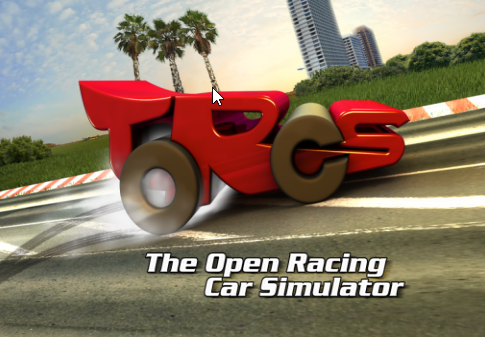
\includegraphics[scale=0.9,width=\columnwidth]{images/torcs.png}
  \caption{Torcs Car simulator and Open Racing environment }
\end{figure}


% You must have at least 2 lines in the paragraph with the drop letter
% (should never be an issue)


\section{Preliminaries}
Reinforcement Learning is part of Machine Learning practices with supervised and unsupervised learning. Unlike these methods, reinforcement learning creates its own data by interacting with environment. There are two main approaches for solving problems via reinforcement learning, value function based and policy based methods. We have implemented both of these approaches with different algorithms. Below is the summary of the studies we have used in this project.

\subsection{Soft Actor-Critic: Off-Policy Maximum Entropy Deep Reinforcement Learning with a Stochastic Actor (SAC) \cite{haarnoja2018soft} \cite{haarnoja2018soft2}}
SAC uses a modified RL objective function using maximum entropy formulation. Algorithm tries to maximize entropy, in addition to policy updates. This way, agent is encouraged to explore unseen and unknown states. There are two Q networks to estimate expected rewards for policy updates. These two networks are used to minimize Q value overshooting like Double Q learning \cite{van2016deep}. Q function is trained with another V function and since these two networks are dependant on each other, some instabilities may occur. To overcome this, SAC utilizes a target value network and updates it with Polyak averaging \cite{polyak1992acceleration}. Since Q values are the policy's target density function, to achieve differentiation, reparameterization trick is used. Overall, Soft Actor Critic with Maximum Entropy Learning is a data efficient and stable algorithm.

\subsection{Rainbow DQN \cite{hessel2018rainbow}}
Rainbow DQN utilizes multiple improvements on DQN \cite{mnih2015human} together. These improvements are;

\begin{itemize}
    \item Double Q Learning \cite{van2016deep} - This method is used to overcome overestimation problem on Q networks.
    \item Priority Experience Replay \cite{schaul2015prioritized} - Experiences for update are picked with a priority. Mostly used parameter for priority is TD error.
    \item Dueling Networks \cite{wang2015dueling} - Sometimes, choosing the exact action does not matter too much, but the value function estimation is still important. This way value is calculated nevertheless.
    \item Noisy Networks \cite{fortunato2017noisy} - Exploration in environments with Q learning mostly depends on action exploration with epsilon greedy methods. Noisy Networks introduces the capability of parameter space exploration. Parameter change drives state and action exploration.
\end{itemize}

These algorithms together forms the Rainbow DQN approach. We have also used C51 output to obtain further improvements \cite{bellemare2017distributional}.

\section{Implementation}

This section emphasizes on our implementation of the studies explained beforehand. We have tried multiple algorithms like PER-DDPG \cite{hou2017novel}, TD3 \cite{fujimoto2018addressing}, SAC, Rainbow DQN, to overcome TORCS problem, and had significant success with two of them, namely SAC and Rainbow DQN. The codebase is heavily borrowed from \url{https://github.com/medipixel/rl_algorithms}.

\subsection{Architecture}

\subsubsection{SAC}
Our neural network architecture for SAC consists of three layers with 512, 256, and 128 weights respectively. We have used linear layers with ReLU activation on hidden layers and gaussian distribution on actions with TanH activation on output layer. We observed improvements on SAC when we have added a single LSTM layer before output layer. Hyper parameters for SAC-LSTM are below:

\begin{itemize}
    \item Gamma: $0.99$
    \item Tau: $10^{-3}$
    \item Batch Size: $32$
    \item Episode Buffer: $10^3$
    \item Actor Learning Rate: $3.10^{-4}$
    \item Value Learning Rate: $3.10^{-4}$
    \item Q Learning Rate: $3.10^{-4}$
    \item Entropy Learning Rate: $3.10^{-4}$
    \item Policy Update Interval: $2$
    \item Initial Random Action: $10^4$
\end{itemize}

We have used auto entropy tuning using log probabilities. Before LSTM, we have also deployed NSTACK mechanism. We serialized 4 past states and used as input. When we noticed that LSTM outperforms NSTACK approach, we have abandoned SAC and NSTACK mechanism.

\subsubsection{Rainbow DQN}
DQN network consists of three layers of 128 weights. The activation functions of hidden layers are ReLU like, SAC architecture, but outputs are 51 atom distribution over Q values, namely C51. As stated before, we are using Noisy-Net for exploration as opposed to epsilon greedy mechanism. Hyper parameters for Rainbow DQN are below:

\begin{itemize}
    \item N-Step: $3$
    \item Gamma: $0.975$
    \item Tau: $10^{-3}$
    \item N-Step Weight Parameter: $1$
    \item N-Step Q Regularization Parameter: $10^{-7}$
    \item Buffer Size: $10^5$
    \item Batch Size: $32$
    \item Learning Rate: $10^{-4}$
    \item Adam Epsilon: $10^{-8}$
    \item Adam Weight Decay: $10^{-7}$
    \item PER Alpha: $0.6$
    \item PER Beta: $0.4$
    \item PER Epsilon: $10^{-6}$
    \item Gradient Clip: $10$
    \item Prefill Buffer Size: $10^{4}$
    \item C51 - V Minimum: $-300$
    \item C51 - V Maximum: $300$
    \item C51 - Atom Size: $1530$
    \item NoisyNet Initial Variance: $0.5$
\end{itemize}

\subsection{Reward Shaping}
Like many TORCS agent developers, we have noticed the fast left right maneuvers on a straight track. We have tried multiple reward functions to stabilize the car. In addition to this, when the agent steers off track and turns backwards, environment resets. This way agent does not try to recover from the state. We have also tried to recover from this.

\subsubsection{Termination}
We have changed some of the termination conditions provided. Our terminal judge starts after 100 timesteps, similar to this, we have provided agent 100 timesteps to recover from turning backwards. This way we want to see agent try to get on track after spins.

\subsubsection{Reward Functions}
The parameters used in reward functions are defined as,
\begin{itemize}
    \item $V_x$: Longitudinal velocity
    \item $V_y$: Lateral velocity
    \item $\theta$: Angle between car and track axis
    \item $trackpos$: Distance between center of the road and car
\end{itemize}

Reward functions we have tried are formulated below. We have noticed that in the original reward function, negative angles with sine penalties become positive. This makes agent biased towards left.

\begin{itemize}
    \item No Trackpos: $V_x \cos\theta - |V_x \sin\theta|$
    \item Trackpos: $V_x \cos\theta - |V_x \sin\theta| - |V_x trackpos|$
    \item EndToEnd \cite{jaritz2018end}: $V_x (\cos\theta - |trackpos|)$
    \item Extra \cite{deeprltorcs}: $V_x \cos\theta - |V_x\sin\theta| - |2V_x\sin\theta trackpos| - V_y \cos\theta$
    \item Sigmoid: $V_x sigmoid(\cos\theta * 3) - V_x \sin\theta - V_y sigmoid(\cos\theta * 3)$
\end{itemize}

We have also further tried penalizing not turning at turns using lidar values. Our agent uses ``Extra'' reward function formulated above. We did not have enough time to throughly test ``Sigmoid'' function, it looks promising to overcome fast maneuvers on a straight track since it soft clips the cosine rewards.

\subsection{Exploration}
Exploration in this environments is done by maximizing entropy in SAC and NoisyNets in DQN algorithm. But learning to utilize brake is a challenge since using brake decreases reward. We have employed Stochastic Braking for this.

\subsubsection{Try-Brake}
Try Brake mechanism is like Stochastic Braking \cite{deeprltorcs}. After a certain amount of timesteps, agent is forced to use brake $10\%$ of the time, again for a certain amount of time. This way we hope that agent will learn to speed up in a straight track and brake before and while turns.

\subsection{Generalization}
We have further added 13 more tracks to train and test on to generalize agent's behaviour on unseen tracks. This way, we try to prevent agent to overfit and memorize the tracks. All added tracks are road tracks. We avoided using Spring track since it is very long.

\subsection{Environments}
We have changed environment action and step functions to make learning easier for agent. Below are two of the implementation and explanations of the environments we have tried.

\subsubsection{Continuous Environment}
In this environment, we have reduced to action size to 2. First action value is used for both accelerating and braking. Since agent won't try to use them together, defining two actions for them is unnecessary. Smaller values than zero are used for brake values and greater values are used for accelerating. Second action value is used for straight forward steering. We use this environment for SAC algorithm.

\subsubsection{Discretized Environment}
Since our DQN algorithm is suitable to discrete actions, we have dicretized action space into 21 actions. There are 7 steering points on 3 modals. First modal is for accelerating and steering, second modal is only steering and last modal is for braking and steering.

\section{Experiements}

% no \IEEEPARstart
We divide our experiements into 3 categories.

\begin{itemize}
    \item Score vs Loss curves
    \item Algorithm Comparisons
    \item Track Comparisons
\end{itemize}
\
For the x axis , We decided to use \textbf{timestep} feature instead of the \textbf{episode} to treat algorithms equally independent of the underlying hardware running simulation.\\

\textbf{SAC Algorithm with LSTM}\

With the SAC algorithm the max speed can reach upto 180 km/h while the average speed is around 125 km/h. These results were obtained around 1.4billion times steps.\

\begin{figure}[hbt!]
  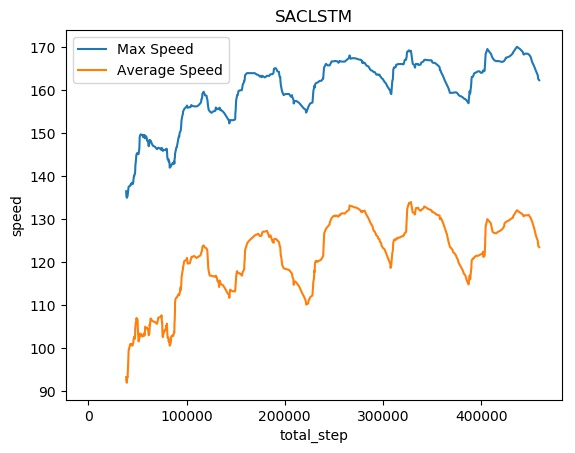
\includegraphics[scale=0.9,width=\columnwidth]{images/graphs/speed_SACLSTM_XUFV9F8G.jpg}
  \caption{Max Speed - Average Speed vs total steps with SACLSTM }
\end{figure}
\
The loss against totals steps are depicted in Figure 3\

\begin{figure}[hbt!]
  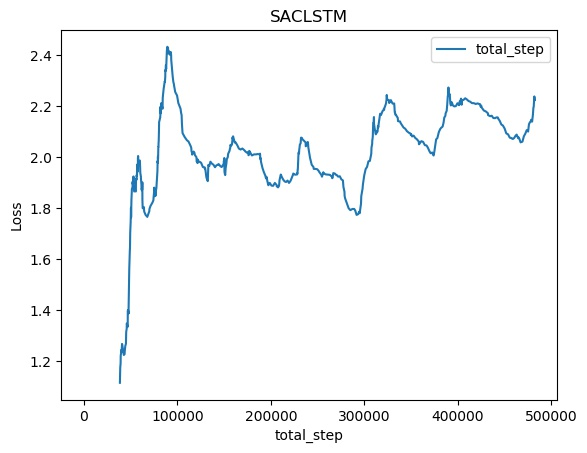
\includegraphics[scale=0.9,width=\columnwidth]{images/graphs/Loss_SACLSTM_W8FAAPZE.jpg}
  \caption{Total Loss vs total steps with SACLSTM }
\end{figure}
\

Finally the Reward curve is shown in Figure 4.\
It is noticable there are steep falls in the Reward around 0.6 billion. This is due to the resume of a previously trained model where some bad rewards are taken.\

\begin{figure}[hbt!]
  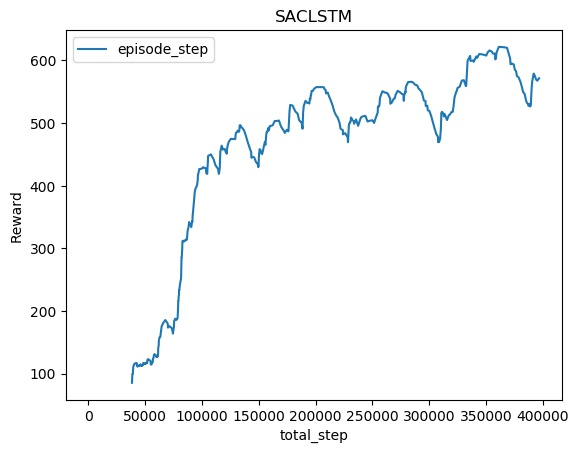
\includegraphics[scale=0.9,width=\columnwidth]{images/graphs/Reward_SACLSTM_ZN8M3NUN.jpg}
  \caption{Reward vs total steps with SACLSTM }
\end{figure}

\textbf{DQN}

We have observed DQN with the following loss and reward figures as in figure 5 and 6.\
\begin{figure}[hbt!]
  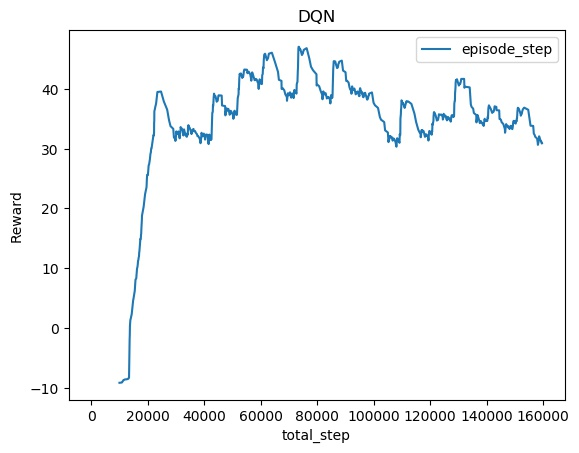
\includegraphics[scale=0.9,width=\columnwidth]{images/graphs/Reward_DQN_EXAB2JN4.jpg}
  \caption{Reward vs total steps with DQN }
\end{figure}

\begin{figure}[hbt!]
  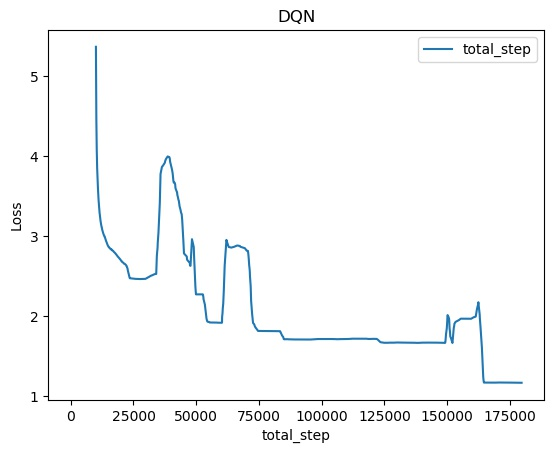
\includegraphics[scale=0.9,width=\columnwidth]{images/graphs/Loss_DQN_P0GOAW9K.jpg}
  \caption{Loss vs total steps with DQN }
\end{figure}


\textbf{Algorithms against Tracks}
We have used 19 different tracks for the training. Some tracks are straightforward like e-track-1 where on the other some of them have difficulties with sharp turns or even gravitational effects.\

The success among those tracks are shown in Figure 7 :

\begin{figure}[hbt!]
  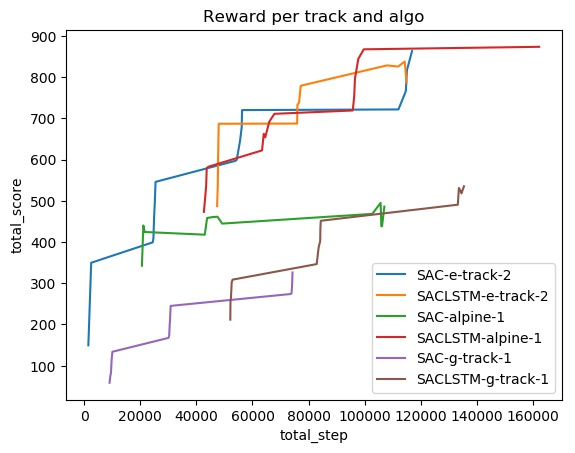
\includegraphics[scale=0.9,width=\columnwidth]{images/graphs/tracks_3Z519A2L.jpg}
  \caption{SAC and SACLSTM algorithms against 3 different tracks }
\end{figure}

Finally the perforance in terms of Max Speed of algorithms in tracks are shown in Figure 8:\


\begin{figure}[hbt!]
  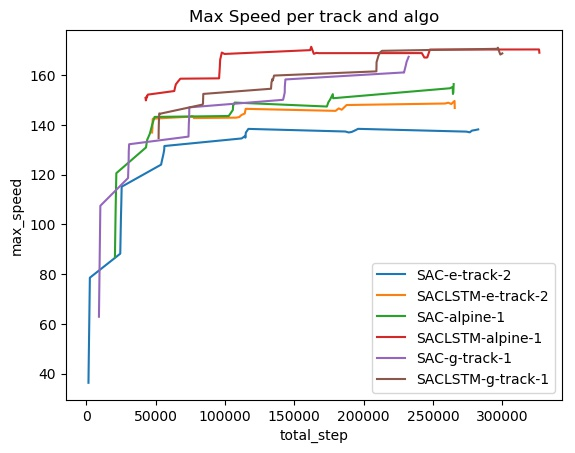
\includegraphics[scale=0.9,width=\columnwidth]{images/graphs/tracks_CGPVM3RT.jpg}
  \caption{SAC and SACLSTM algorithms against 3 different tracks }
\end{figure}



% no \IEEEPARstart


\section{Discussions}
TODO
% no \IEEEPARstart









% trigger a \newpage just before the given reference
% number - used to balance the columns on the last page
% adjust value as needed - may need to be readjusted if
% the document is modified later
%\IEEEtriggeratref{8}
% The "triggered" command can be changed if desired:
%\IEEEtriggercmd{\enlargethispage{-5in}}

% references section

% can use a bibliography generated by BibTeX as a .bbl file
% BibTeX documentation can be easily obtained at:
% http://mirror.ctan.org/biblio/bibtex/contrib/doc/
% The IEEEtran BibTeX style support page is at:
% http://www.michaelshell.org/tex/ieeetran/bibtex/
%\bibliographystyle{IEEEtran}
% argument is your BibTeX string definitions and bibliography database(s)
%\bibliography{IEEEabrv,../bib/paper}
%
% <OR> manually copy in the resultant .bbl file
% set second argument of \begin to the number of references
% (used to reserve space for the reference number labels box)
\bibliographystyle{IEEEtran}
\bibliography{main}




% that's all folks
\end{document}


